%%%%%%%%%%%%%%%%%%%%%%%%%%  ltexpprt_twocolumn.tex  %%%%%%%%%%%%%%%%%%%%%%%%%%%%%%%%
%
% This is ltexpprt_twocolumn.tex, an example file for use with the SIAM LaTeX2E
% Preprint Series macros. It is designed to provide two-column output.
% Please take the time to read the following comments, as they document
% how to use these macros. This file can be composed and printed out for
% use as sample output.

% Any comments or questions regarding these macros should be directed to:
%
%                 Donna Witzleben
%                 SIAM
%                 3600 University City Science Center
%                 Philadelphia, PA 19104-2688
%                 USA
%                 Telephone: (215) 382-9800
%                 Fax: (215) 386-7999
%                 e-mail: witzleben@siam.org


% This file is to be used as an example for style only. It should not be read
% for content.

%%%%%%%%%%%%%%% PLEASE NOTE THE FOLLOWING STYLE RESTRICTIONS %%%%%%%%%%%%%%%

%%  1. There are no new tags.  Existing LaTeX tags have been formatted to match
%%     the Preprint series style.
%%
%%  2. Do not change the margins or page size!  Do not change from the default
%%     text font!
%%
%%  3. You must use \cite in the text to mark your reference citations and
%%     \bibitem in the listing of references at the end of your chapter. See
%%     the examples in the following file. If you are using BibTeX, please
%%     supply the bst file with the manuscript file.
%%
%%  4. This macro is set up for two levels of headings (\section and
%%     \subsection). The macro will automatically number the headings for you.
%%
%%  5. No running heads are to be used for this volume.
%%
%%  6. Theorems, Lemmas, Definitions, Equations, etc. are to be double numbered,
%%     indicating the section and the occurrence of that element
%%     within that section. (For example, the first theorem in the second
%%     section would be numbered 2.1. The macro will
%%     automatically do the numbering for you.
%%
%%  7. Figures and Tables must be single-numbered.
%%     Use existing LaTeX tags for these elements.
%%     Numbering will be done automatically.
%%
%%  8. Page numbering is no longer included in this macro.
%%     Pagination will be set by the program committee.
%%
%%
%%%%%%%%%%%%%%%%%%%%%%%%%%%%%%%%%%%%%%%%%%%%%%%%%%%%%%%%%%%%%%%%%%%%%%%%%%%%%%%



\documentclass[twoside,leqno,twocolumn]{article}

% Comment out the line below if using A4 paper size
\usepackage[letterpaper]{geometry}

\usepackage{ltexpprt}
\usepackage{hyperref}
\usepackage{lipsum}

\usepackage{graphicx}
\usepackage{amssymb}
\usepackage{bbm}
\usepackage{amsmath}
\usepackage{lscape}
\usepackage{subcaption}
\usepackage{mwe}
\usepackage{dirtytalk}
\usepackage{todonotes}
\usepackage{booktabs}
\DeclareMathOperator{\knn}{\textit{k}\text{NN}}
\newcommand{\AZ}[1]{\todo[color=blue!20,author=Zimek]{#1}}
\newcommand{\JG}[1]{\todo[color=green!20,author=Goettcke]{#1}}
\newcommand{\CB}[1]{\todo[color=red!20,author=Bellinger]{#1}}
\newcommand{\PB}[1]{\todo[color=orange!20,author=Branco]{#1}}
\begin{document}

%
\newcommand\relatedversion{}
\renewcommand\relatedversion{\thanks{The full version of the paper can be accessed at \protect\url{https://arxiv.org/abs/1902.09310}}} % Replace URL with link to full paper or comment out this line


%\setcounter{chapter}{2} % If you are doing your chapter as chapter one,
%\setcounter{section}{3} % comment these two lines out.

%\title{\Large Improving classifier performance estimation in imbalanced learning problems using Tomek Links}
\title{\Large An Interpretable Measure of Dataset Complexity for Imbalanced Classification Problems}
\author{Jonatan Møller Nuutinen Gøttcke \thanks{University of Southern Denmark}
\and Colin Bellinger \thanks{National Research Council of Canada} 
\and Paula Branco \thanks{University of Ottawa}
\and Arthur Zimek \thanks{University of Southern Denmark}}

\date{\today}

\maketitle

% Copyright Statement
% When submitting your final paper to a SIAM proceedings, it is requested that you include
% the appropriate copyright in the footer of the paper.  The copyright added should be
% consistent with the copyright selected on the copyright form submitted with the paper.
% Please note that "20XX" should be changed to the year of the meeting.

% Default Copyright Statement
\fancyfoot[R]{\scriptsize{Copyright \textcopyright\ 2023 by SIAM\\
Unauthorized reproduction of this article is prohibited}}

% Depending on which copyright you agree to when you sign the copyright form, the copyright
% can be changed to one of the following after commenting out the default copyright statement
% above.

%\fancyfoot[R]{\scriptsize{Copyright \textcopyright\ 20XX\\
%Copyright for this paper is retained by authors}}

%\fancyfoot[R]{\scriptsize{Copyright \textcopyright\ 20XX\\
%Copyright retained by principal author's organization}}

%\pagenumbering{arabic}
%\setcounter{page}{1}%Leave this line commented out.

\begin{abstract} \small\baselineskip=9pt The class imbalance problem is associated with harmful classification bias and presents itself in a wide variety of important applications of supervised machine learning. Measures have been developed to determine the imbalance complexity of datasets with imbalanced classes. The most common such measure is the Imbalance Ratio (IR). It is, however, widely accepted that the complexity of a classification task is the combined result of class imbalance and other factors, such as class overlap. Thus, in order to accurately assess the complexity of a problem, the data complexity measures ought to account for more than the simple IR. In this paper we demonstrate that IR has a weak correlation with classifier performance in terms of macro averaged recall, gmean score, and precision. Other more complete measures such as the adapted N1 and N3 measures use neighborhood information to assess overlap. These measures show a strong negative correlation with classifier performance, but their reported values are hard to interpret. This motivates a new measure which estimates overlap complexity and returns a value with a clear interpretation. Here we propose such a measure based on the number of minority instances entangled in a Tomek Link. The proposed measure is evaluated on a large selection of synthetic and real datasets and is found to be as good as or better than the best competitors in terms of its negative correlation with respect to mean classifier performance.
\end{abstract}

\section{Introduction} \label{sec:introduction}
In the field of supervised learning one of the most persistent issues is imbalanced data distributions. This is commonly referred to as the class imbalance problem. Imbalanced data distributions often lead to a bias towards predicting the majority class or classes, which in most cases is very undesired. Describing a datasets complexity accurately, in terms of some classification problem gives us some interesting possibilities. Before building a model on a dataset, it is important to have knowledge about the dataset, to know how to approach it, and which potential pitfalls are present. Therefore we must have a way of describing the severity of mechanisms which make classification tasks complex. When a new method is proposed, which claims to handle such a complexity, this measure can be used to determine which datasets are relevant in the benchmark. In everyday classification problems it is also relevant to have a tool which can assist us in checking the type of complexity that is hindering classifier performance. In many papers on the imbalance problem, where a larger experimental framework is made the method of determining whether class imbalance is present is done by reporting the Imbalance Ratio (IR).\JG{Insert citations} It can therefore be seen as the de facto standard when it comes to measuring the severity of the class imbalance problem. 
The Imbalance Ratio is defined in Equation \ref{eq:imbalance_ratio} and gives an easy understanding of the level of imbalance. It is the ratio between the number of points in the largest majority class and the smallest minority class. $\mathcal{D}$ is the domain containing all instances within the dataset, and $C_{maj}$ and $C_{min}$ is respectively the majority and minority class subsets of the domain. \CB{Consider linking the need for good imbalance complexity metrics to meta-learning and auto-ml}
\CB{TODO There are papers that theoretically and empirically compare the implications of g-mean, AUC and FM for classifier evaluation. We should consider having a few sentences on these to motivate our focus on FM. Also, in some applications, of course, FM/P/R are just more appropriate metrics (e.g. information retrieval, medical diagnosis) we should mention this too.}
\begin{equation}
    \label{eq:imbalance_ratio}
    \text{IR}(\mathcal{D})=\frac{|C_{maj}|}{|C_{min}|}
\end{equation}

Several works have explored statistical measures to find an alternative to the class imbalance ratio such as the Imbalance Degree \cite{DBLP:journals/prl/Ortigosa-Hernandez17}, or LRID~\cite{DBLP:journals/prl/ZhuWMWX18}, which both do a deeper analysis of the class distributions. A measure called the Adjusted Imbalance Ratio \cite{DBLP:journals/prl/ZhuGX20} scale the imbalance ratio given the number of discriminative features. Common for these measures is that they do not use any information about the overlap between data from imbalanced class distributions, and even in the most highly imbalanced case two classes can be separated by a straight line, if there is no overlap. In Luengo et al. \cite{luengo2011addressing} they study how 12 different dataset complexity measures are affected by class imbalance preprocessing. They conclude that IR is insufficient to predict if one of the two classifiers is going to perform well or not. In this paper we arrive at the same conclusion. The correlation we find between IR and classifier performance can be seen in Figure~\ref{fig:ir_dataset_plot}.
\begin{figure}[tbp]
\centering
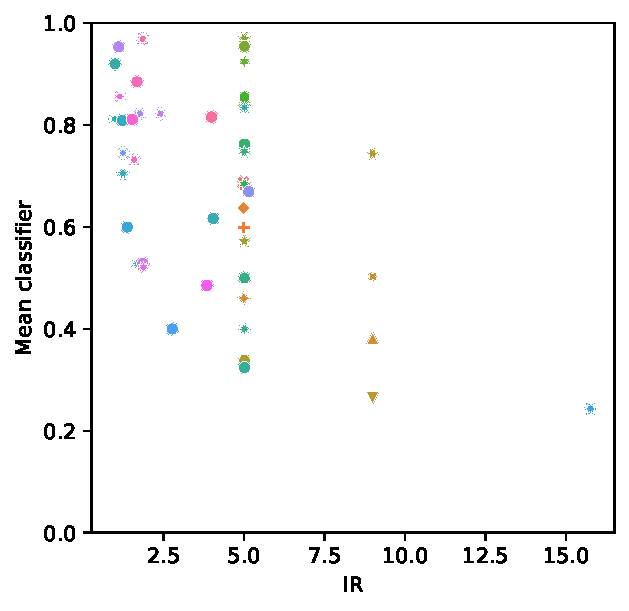
\includegraphics[width=0.9\columnwidth]{plots/dataset_plots/siam_full_plot_IR.pdf}
\caption{The correlation between the imbalance ratio and a mean classifiers performance in terms of macro averaged recall.}
\label{fig:ir_dataset_plot}
\end{figure}
Since the most commonly reported measure for determining class imbalance complexity i.e. IR does not imply complexity in the classification task, it is necessary to explore this field in depth, and find alternatives. 
A considerable effort in recent years has been put into broadening our understanding of the origin of complexity in class imbalanced scenarios. Recently the presence of the imbalance ratio between classes as well as their overlap has been studied in several works \cite{DBLP:journals/isci/BarellaGSLC21,raj2016towards,santos2022joint}. Even though the new measures are much more correlated with a degradation in classifier performance none of them have succeeded in replacing IR as the de facto standard measure of imbalance complexity. That might be because IR has a simple interpretation. In Section~\ref{sec:related_work} we introduce the measures, we consider the nearest neighbors of the proposed measure, in this research field. In Section~\ref{sec:experimental_evaluation} we introduce the experimental framework used to evaluate the measures, and present our findings. In Section~\ref{sec:discussion} we discuss several findings derived from this research project, and observations about the state of and direction the field. Finally in \ref{sec:conclusion} we conclude the paper. The contributions in this paper is threefold. We define a new measure to the field of complexity measures for imbalanced datasets with as good performance as the former best performers, while being much easier to interpret. We make a series of synthetic datasets available, which have been described in multiple papers \cite{santos2022joint, DBLP:conf/ida/MercierSASSS18}, as well as new datasets, which tests the local imbalance problem. We supply efficient Python implementations of all measures described in this paper, that unlike the existing implementations operate in the popular Scikit-Learn style. \JG{Start adding all the citations.}\JG{It feels like there's missing something about measures not using nearest neighbors like the L and F measures}

%TODO Conider linking the need for good imbalance complexity metrics to meta-learning and auto-ml
%TODO There are papers that theoretically and empirically compare the implications of g-mean, AUC and FM for classifier evaluation. We should consider having a few sentenses on these to motivate our focus on FM. Also, in some applications, of course, FM/P/R are just more appropriate metrics (e.g. information retrival, medical diagnosis) we should mention this too. 


\section{Related Work}
\label{sec:related_work}
Most of the performant dataset complexity measures in the imbalanced classification problem space is based on nearest neighbors. 
In Barella et al. \cite{DBLP:journals/isci/BarellaGSLC21} \emph{Assessing the data complexity of imbalanced datasets} they adapt a selection of existing data complexity measures, to account for class imbalance. Through their very thorough experimental framework, they find some extremely robust measures where possibly the two most noticeable measures are their adaptation of N1 and N3.
\begin{equation}
    \label{eq:n1}
     \text{N1}_{c_1}(T)=\frac{1}{n_{c_{1}}}\sum_{i=1}^{n_{c_{1}}}\text{I}((x_i^{c_1},x_j)\in \text{MST} \wedge c_1 \neq y_j)
\end{equation}
The adapted \emph{N1} measure as described in \ref{eq:n1} builds a minimum spanning tree (MST) over the dataset, and returns the fraction of edges connecting vertices from class $c_1$ to vertices of class $y_j$ where  $y_j \neq c_1$. The identity function $\text{I}$ in the equation is 1 if the inner expression is true.

\begin{equation}
    \label{eq:n3}
    \text{N3}_{c_1}(T)=\frac{\sum_{i=1}^{n}\text{I}(\text{NN}(x_i^{c_1}) \neq c_1)}{n_{c_{1}}}
\end{equation} The adapted N3 measure returns the leave one out error rate of the first nearest neighbor classifier for class $c_1$. Here $\text{NN}(x_i)$ returns the label of the nearest neighbor of instance $x_i$. 

For both the adapted N1 and N3 which altered from the original versions to be class specific measures, the aggregate measure for the entire dataset is found by taking the mean of each measure. 

Mercier et al. \cite{DBLP:conf/ida/MercierSASSS18} presents two measures dubbed Degree IR (degIR) and Overlap degree (degOver) which measures the complexity as a function of local imbalance and overlap. The overlap is determined by the $5\text{NN}$ set. If the 5-nearest neighbors of an instance belong to the same class as the instance, then the instance is not in a region of overlap, otherwise it is.  

The number of points from the minority class, that are in an overlapping region is defined as $n_{min\_over}$ and the number of points from the majority class, that are in an overlapping region is defined as $n_{maj\_over}$. Then the overlap degree is defined as shown in Equation \ref{eq:overlap degree}
\begin{equation}
\label{eq:overlap degree}
\text{degOver}(\mathcal{D})=\frac{n_{min\_over} + n_{maj\_over}}{n}
\end{equation}
The degree IR after normalization is defined as \ref{eq:degIR}
\begin{equation}
\label{eq:degIR}
\text{degIR}(\mathcal{D})=1-\frac{n_{min\_over}}{\frac{n}{2}}=1-\frac{2n_{min\_over}}{n}
\end{equation} \JG{Currently I did not include the degIR measure in the results, maybe we should include more results in the tables, and just put the plots for the best ones}

\section{Tomek link complexity measure}
\label{sec:tlcm_introduction}
Here we define a measure based on the Tomek Links \cite{Tomek76} commonly used in undersampling\JG{Citation}. Tomek Links are pairs of mutual nearest neighbors of opposite classes, as described in Equation \ref{eq:tomek_links} where $x_i$ and $x_j$ are instances belonging to class $y_i$ and $y_j$. The point $x_k$ is any arbitrary point in the dataset. $C_{min}$ is the set of minority class instances. \JG{Do we talk about dimensionality} \JG{Mention how to compute for multiclass}
\begin{align}
    d(x_i,x_j) <&\ d(x_i,x_k) \label{eq:tomek_links} \\
    \nonumber d(x_i,x_j) <&\ d(x_j,x_k) \\
    \nonumber y_i=C_{min} \lor&\ y_j = C_{min} \\
    \nonumber y_i \neq&\ y_j 
\end{align}
Given the definition of a Tomek Link in Equation \ref{eq:tomek_links} the measure described in Equation \ref{eq:tlcm} calculates the proportion of minority instances entangled in a Tomek Link. 
\begin{equation}
    \label{eq:number_of_tomek_links}
    \text{TLS}(\mathcal{D}) = \sum_{i \in C_{min}}\ \sum_{j \in \mathcal{D} \setminus C_{min}} TL(x_i,x_j)
\end{equation}

\begin{equation}
    \label{eq:tlcm}
    \text{TLCM}( \mathcal{D} )=\frac{\text{TLS}(\mathcal{D})}{|C_{min}|}
\end{equation}
In Equation \ref{eq:number_of_tomek_links} the number of Tomek links in the dataset is defined as $\text{TLS}$. Here $\mathcal{D}$\JG{Is D this first introduced here?} is the set of all instances in the domain and $TL$ is the identity function that returns $1$, if $x_i$ and $x_j$ form a Tomek link according to definition \ref{eq:tomek_links}. The cardinality $|C_{min}|$ defines the number of points within the set of minority instances. The measure proposed in this paper is defined as the Tomek Link Complexity Measure ($\text{TLCM}$) and is defined in Equation \ref{eq:tlcm}.
Tomek Links on the decision boundary adds to the complexity e.g. if we have two uniform linearly separable distributions parallel to each other as in Figure~\ref{fig:uniform_only_boundary}, then a measure based on the first few nearest neighbors of the minority points will almost always have the majority class in the decision set. Tomek Links ensures this is not the case, since the two instances have to be mutual nearest neighbors, which improves this nearest neighbor based approach ability at catching separability. The $\text{TLCM}$ measures can be summarized as the percentage of instances from the minority, entangled in a Tomek Link.  
\JG{Maybe insert an illustration of what a Tomek Link is}

\section{Experimental Evaluation}
\label{sec:experimental_evaluation}
\subsection{Datasets} \JG{Is ImbCol package here anywhere?}
A subset of the synthetic datasets used in this paper are used in both Mercier et al. \cite{DBLP:conf/ida/MercierSASSS18} and Santos et al. \cite{santos2022joint}. These datasets were rebuild using the adapted dataset generator from \cite{santos2022joint} and the dataset generator from Goettcke~\cite{DSPipe}. In addition we added the \emph{local imbalance} dataset as well as the \emph{uniform only boundary} dataset. The datasets \emph{02a} and \emph{02b} Figure \ref{fig:02a} and \ref{fig:02b} test the algorithms ability to predict groups within a noisy background distribution. Notice however that there are no noisy points within the subcluster distributions. The \emph{03subcl5} dataset Figure \ref{fig:03subcl5} tests 5 sub-clusters within a noisy background distribution in the same way as \emph{02a} and \emph{02b}, but the density of the clusters becomes smaller with the top one being the most dense, and the bottom one being the least dense. The \emph{clover} dataset Figure \ref{fig:clover} increases the size of the decision boundary, as well as testing the classifiers ability to handle a non Gaussian distribution. The \emph{paw3} dataset shown in Figure~\ref{fig:paw3ob} tests the classifiers ability to predict borderline minority instances from a multi-modal minority distribution. The \emph{paw3} \emph{border dense center} is used in other papers, but it is the authors belief that this tests the same problem as dataset \emph{02a}.
The Gaussian overlap datasets tests a basic type of overlap, where two Gaussians are placed close enough to each other, to have some instances falling into the span of the neighbour distribution. Here it is only shown for the case, where the means are respectively 1 and 4 standard deviations apart as shown in Figure \ref{fig:synthetic_dataset_gaussian_1} and \ref{fig:synthetic_dataset_gaussian_4}, but are also evaluated with 2 and 3 standard deviations. \JG{Since we have all of these datasets we should look at the performance in detail, and locate some of the datasets on the performacne plots}
\begin{figure}{}
    \centering
    \begin{subfigure}[t]{0.24\textwidth}
        \centering
        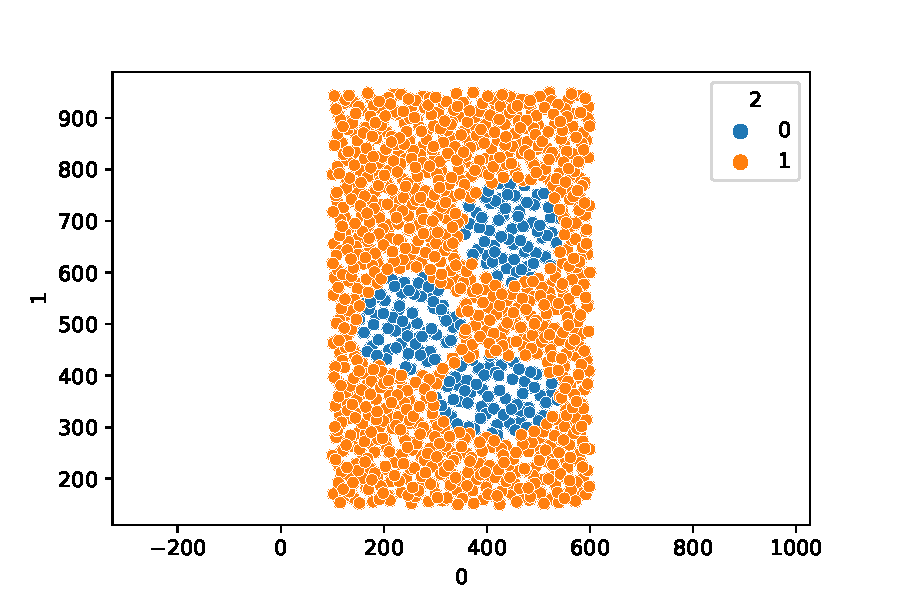
\includegraphics[width=\textwidth]{plots/synthetic_dataset_visualizations/02a.csv.pdf}
        \caption[]%
        {{\small 02a}}    
        \label{fig:02a}
    \end{subfigure}
    \begin{subfigure}[t]{0.24\textwidth}  
        \centering 
        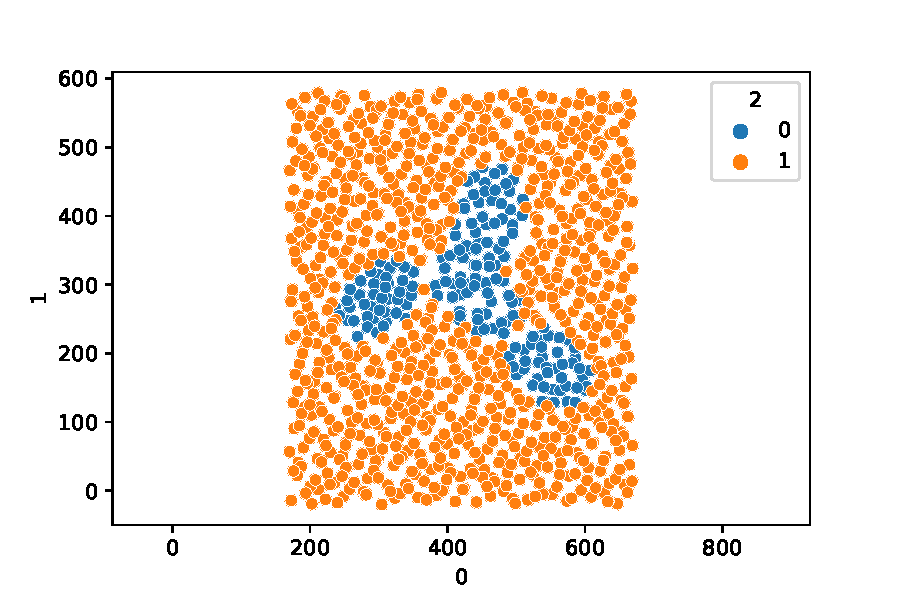
\includegraphics[width=\textwidth]{plots/synthetic_dataset_visualizations/02b.csv.pdf}
        \caption[]%
        {{\small 02b}}    
        \label{fig:02b}
    \end{subfigure}
    \vskip\baselineskip
    \begin{subfigure}[t]{0.24\textwidth}  
        \centering 
        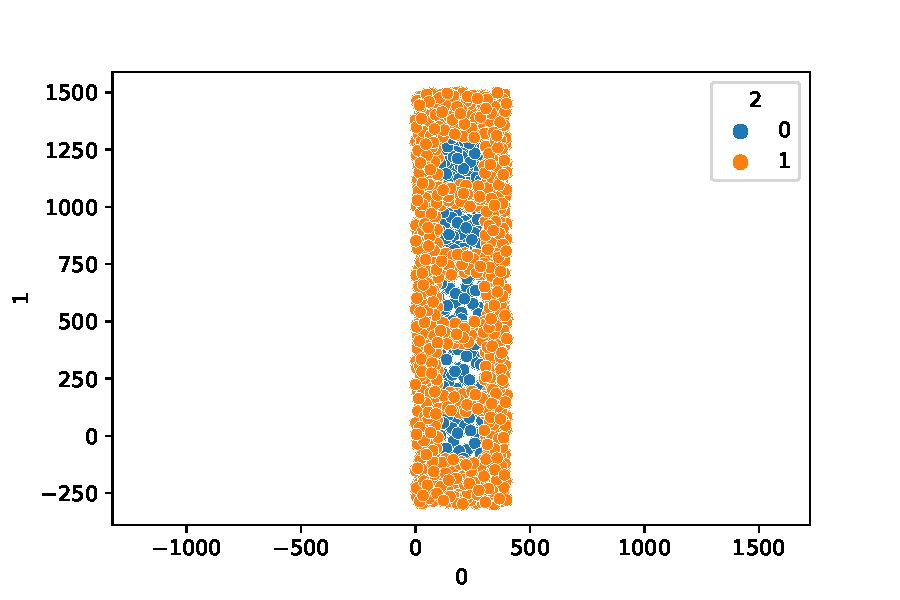
\includegraphics[width=\textwidth]{plots/synthetic_dataset_visualizations/03subcl5.csv.pdf}
        \caption[]%
        {{\small 03subcl5}}    
        \label{fig:03subcl5}
    \end{subfigure}
    \begin{subfigure}[t]{0.24\textwidth}   
        \centering 
        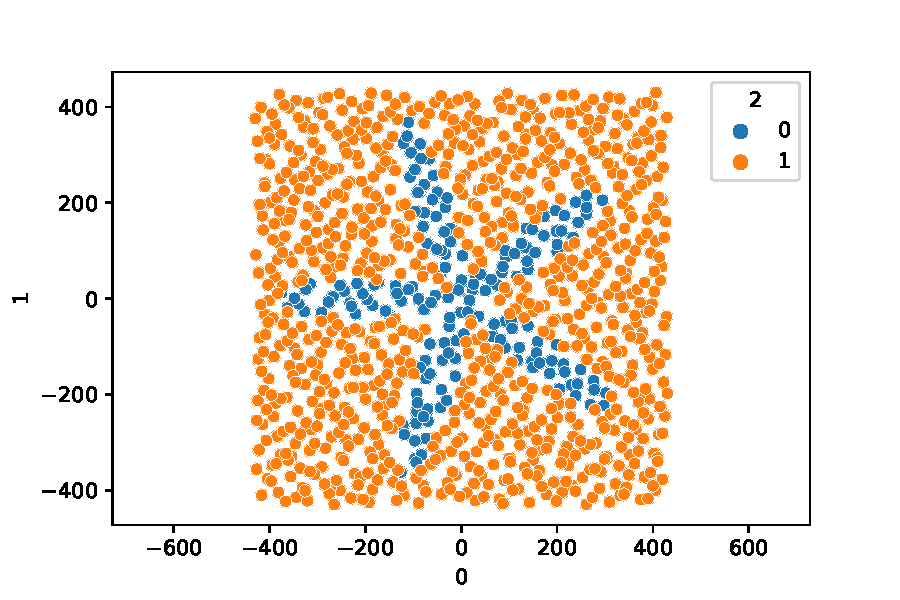
\includegraphics[width=\textwidth]{plots/synthetic_dataset_visualizations/04clover5.csv.pdf}
        \caption[]%
        {{\small 04clover5}}    
        \label{fig:clover}
    \end{subfigure}
    \vskip\baselineskip
    \begin{subfigure}[b]{0.24\textwidth}   
        \centering 
        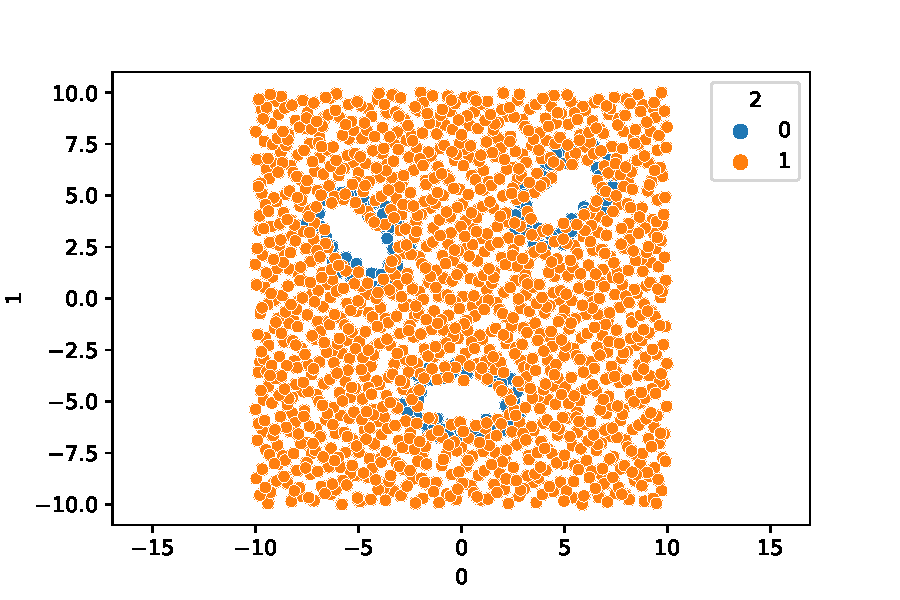
\includegraphics[width=\textwidth]{plots/synthetic_dataset_visualizations/paw3-2d-only-border.csv.pdf}
        \caption[]%
        {{\small paw3 only border}}    
        \label{fig:paw3ob}
    \end{subfigure}
    \begin{subfigure}[b]{0.24\textwidth}   
        \centering 
        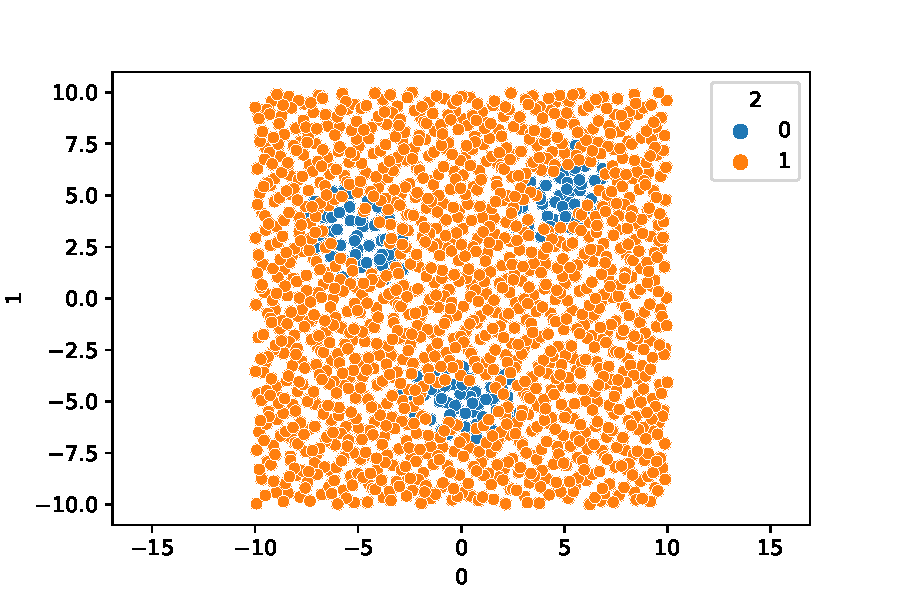
\includegraphics[width=\textwidth]{plots/synthetic_dataset_visualizations/paw3-2d-border-dense-center.csv.pdf}
        \caption[]%
        {{\small paw3 border dense center}}    
        \label{fig:paw3bdc}
    \end{subfigure}
    \begin{subfigure}[b]{0.24\textwidth}
        \centering
        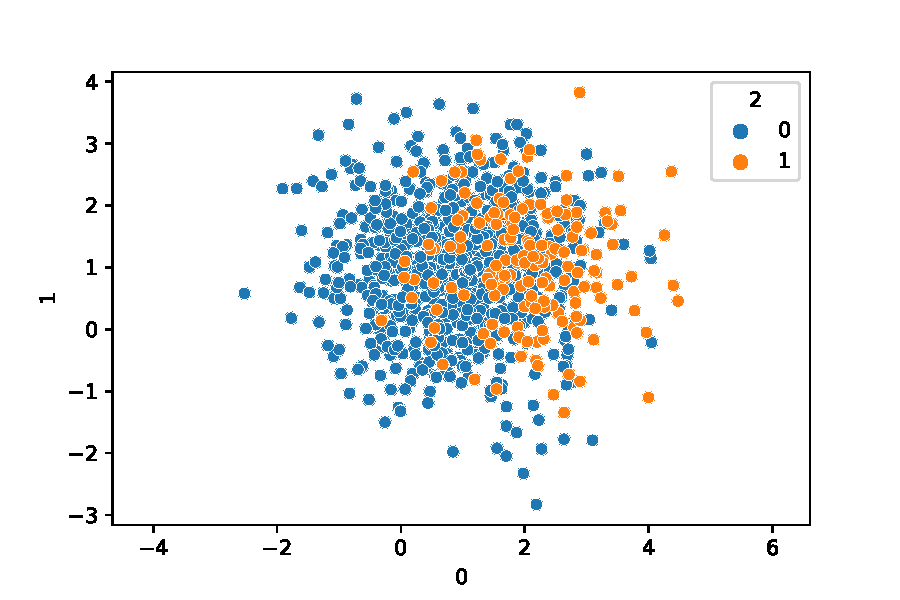
\includegraphics[width=\textwidth]{plots/synthetic_dataset_visualizations/gaussian_overlap_0.83_0.17_1000_1_1.csv.pdf}
        \caption[Network2]%
        {{\small Gaussian overlap 1 standard deviations apart.}}    
        \label{fig:synthetic_dataset_gaussian_1}
    \end{subfigure}
    \hfill
    \begin{subfigure}[b]{0.24\textwidth}  
        \centering 
        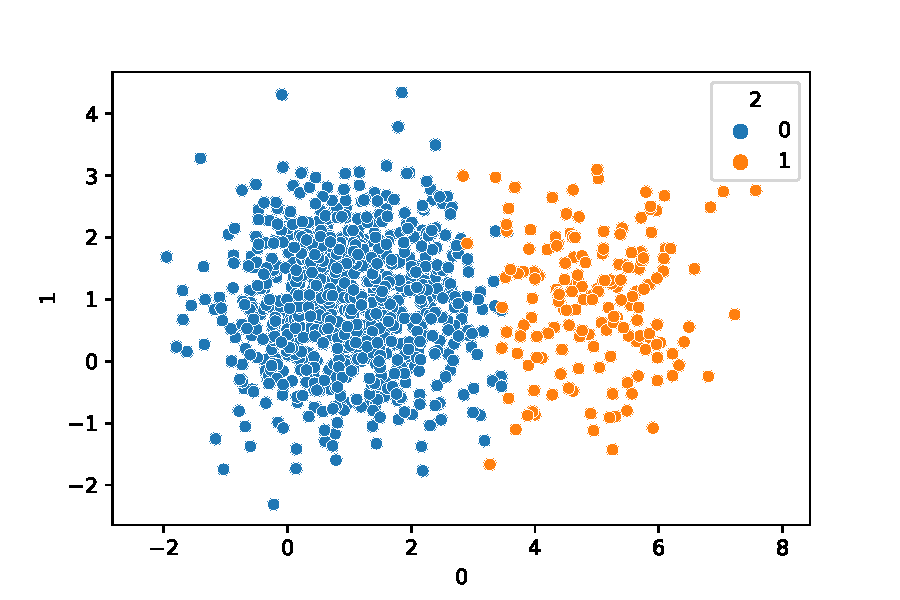
\includegraphics[width=\textwidth]{plots/synthetic_dataset_visualizations/gaussian_overlap_0.83_0.17_1000_1_4.csv.pdf}
        \caption[]%
        {{\small Gaussian overlap 4 standard deviations apart.}}    
        \label{fig:synthetic_dataset_gaussian_4}
    \end{subfigure}
    \caption[]{\label{fig:synthetic-datasets-one} A subset of the synthetic datasets used in the experimental evaluation.}
\end{figure} \CB{Ensure that the plots have axis-labels reasonably close to the size of the font}
Overlap  comes in many forms as shown in \cite{santos2022joint} and one of the forms, that were not present in the existing dataset lineup was a local imbalance problem, where only a part of the dataset is in an overlapping region. This was created by making one uniform majority distribution, and two connected uniform minority distributions. The two uniform minority distributions have different densities to change the local imbalance degree. The overall imbalance ratio between minority and majority will however not be altered by a change in the local imbalance degree, as fewer points in the overlapping distribution, just results in more points in the non-overlapping distribution.\JG{Are there some datasets where n1/3 or TLCM does not work well, and can we explain why? }
\begin{figure} 
    \centering
    \vskip\baselineskip
    \begin{subfigure}[b]{0.24\textwidth}  
        \centering 
        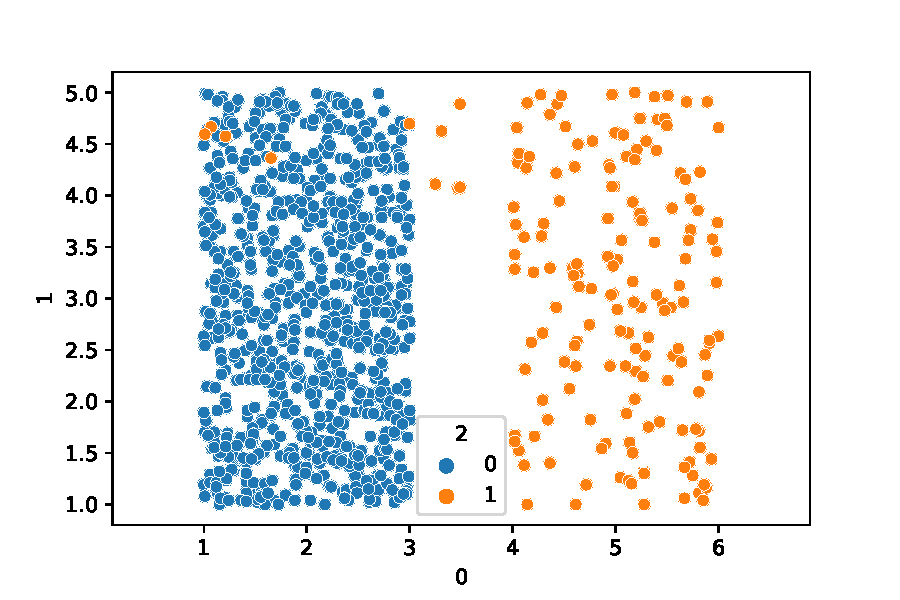
\includegraphics[width=\textwidth]{plots/synthetic_dataset_visualizations/local_imbalance_degree_0.83_0.17_0.05_1000.csv.pdf}
        \caption[]%
        {{\small Local imbalance degree with an IR of 5, and 5 percent of the minority data in the local overlap region.}}    
        \label{fig:local_imbalance-degree_5_percent}
    \end{subfigure}
    \hfill
    \begin{subfigure}[b]{0.24\textwidth}   
        \centering 
        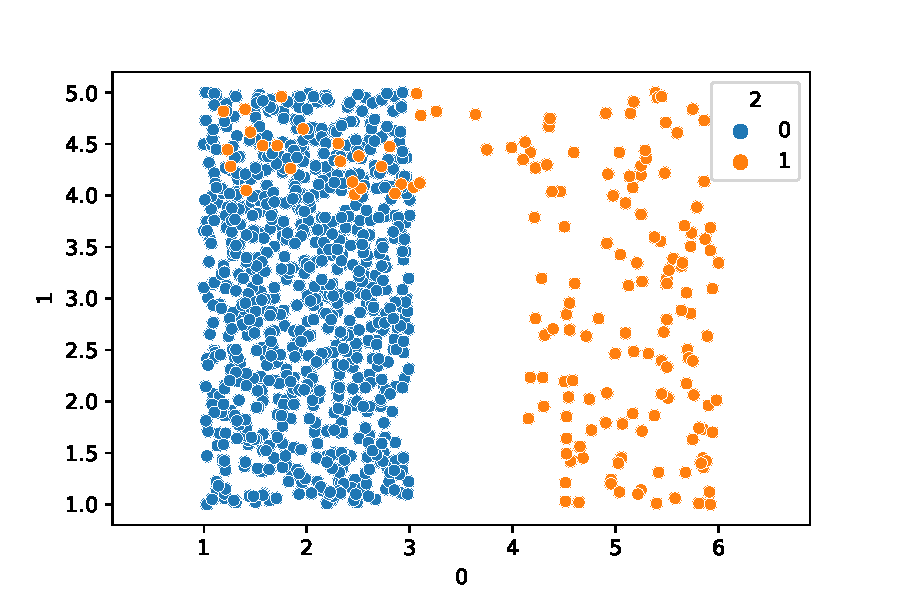
\includegraphics[width=\textwidth]{plots/synthetic_dataset_visualizations/local_imbalance_degree_0.83_0.17_0.2_1000.csv.pdf}
        \caption[]%
        {{\small Local imbalance degree with an IR of 5, and 20 percent of the minority data in the local overlap region.}}    
        \label{fig:local_imbalance-degree_20_percent}
    \end{subfigure}
    \vskip\baselineskip
    \begin{subfigure}[b]{0.24\textwidth}   
        \centering 
        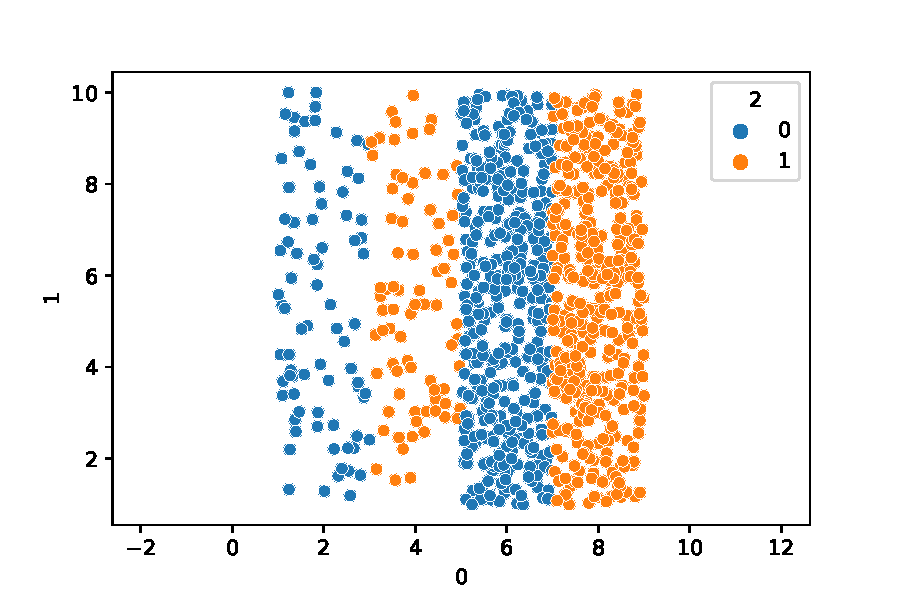
\includegraphics[width=\textwidth]{plots/synthetic_dataset_visualizations/multi_modal_no_overlap_0.83_0.17_1000.csv.pdf}
        \caption[]%
        {{\small multi modal no overlap}}    
        \label{fig:multi_modal_no_overlap}
    \end{subfigure}
    \hfill
    \begin{subfigure}[b]{0.24\textwidth}   
        \centering 
        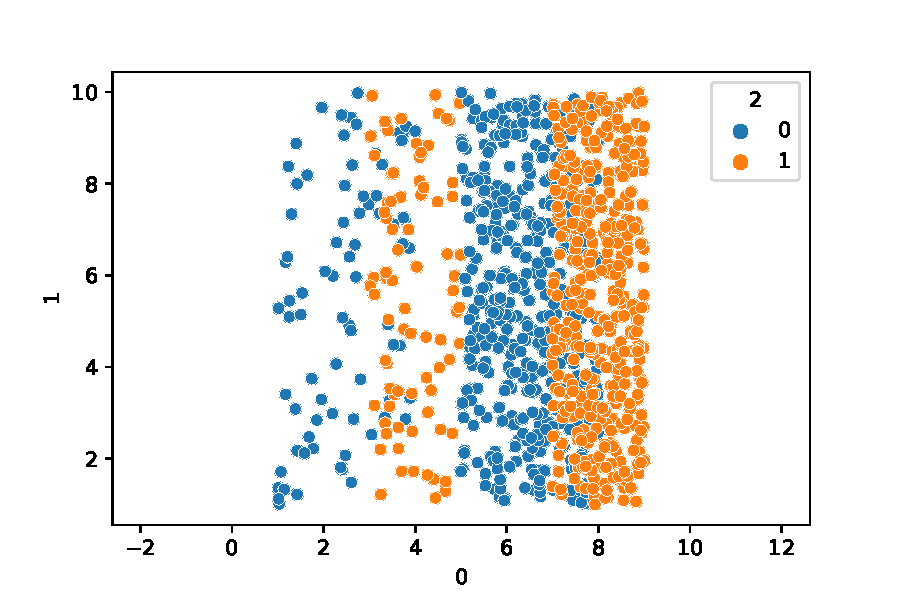
\includegraphics[width=\textwidth]{plots/synthetic_dataset_visualizations/multi_modal_overlap_0.83_0.17_1000.csv.pdf}
        \caption[]%
        {{\small multi modal with overlap}}    
        \label{fig:multi_modal_with_overlap}
    \end{subfigure}
    \vskip\baselineskip
    \begin{subfigure}[b]{0.4\textwidth}   
        \centering 
        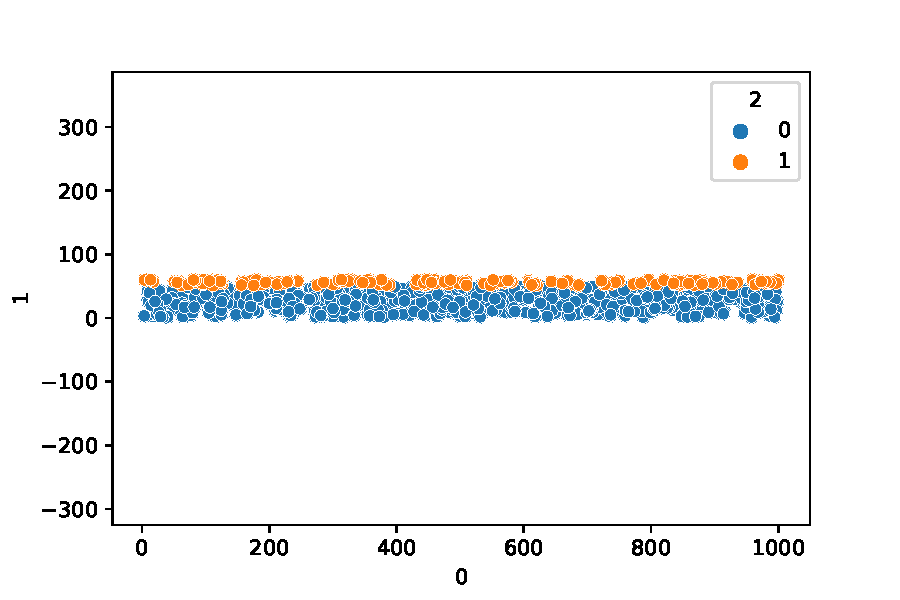
\includegraphics[width=\textwidth]{plots/synthetic_dataset_visualizations/uniform_only_boundary_no_overlap_0.83_0.17_1000.csv.pdf}
        \caption[]%
        {{\small Uniform only boundary}}    
        \label{fig:uniform_only_boundary}
    \end{subfigure}
    \begin{subfigure}[b]{0.24\textwidth}
        \centering
        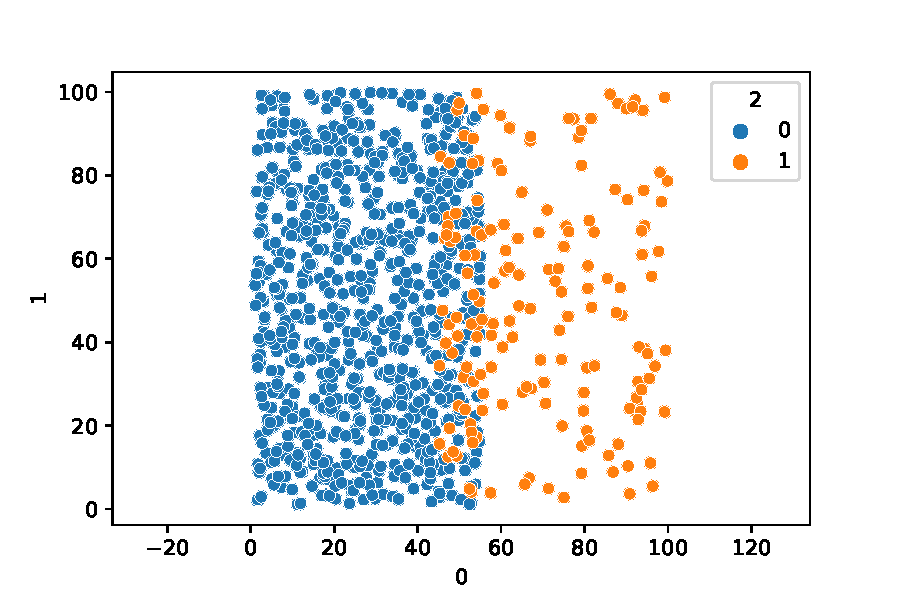
\includegraphics[width=\textwidth]{plots/synthetic_dataset_visualizations/uniform_overlap_0.83_0.17_10_1000.csv.pdf}
        \caption[Network2]%
        {{\small 10\% overlap.}}    
        \label{fig:unform_overlap_10}
    \end{subfigure}
    \hfill
    \begin{subfigure}[b]{0.24\textwidth}  
        \centering 
        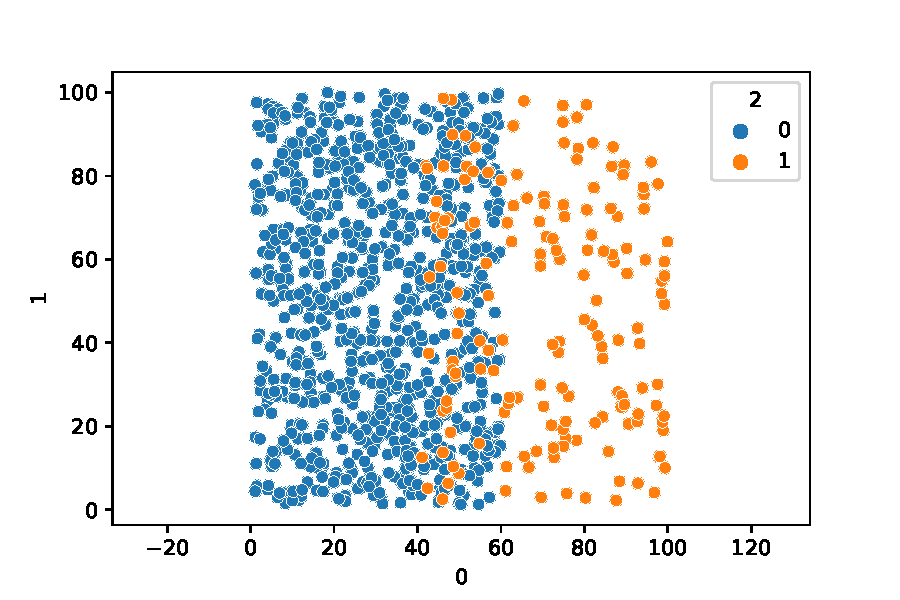
\includegraphics[width=\textwidth]{plots/synthetic_dataset_visualizations/uniform_overlap_0.83_0.17_20_1000.csv.pdf}
        \caption[]%
        {{\small 20\% overlap.}}    
        \label{fig:uniform_overlap_20}
    \end{subfigure}
    \caption[]
    {\small A series synthetic datasets highlighting different overlap scenarios, and dataset complexities. The imbalance ratio in all of the illustrated datasets was $\text{IR}=5$.} 
    \label{fig:mean and std of nets}
\end{figure}
In addition to the synthetic datasets a set of commonly used datasets from the Keel repository \JG{Insert citation} was chosen. These datasets were chosen because of their popularity in the class imbalance literature but also based on three constraints, the number of instances should be smaller than ten thousand, they are binary problems, and the imbalance ratio is greater than 1.1.   

\subsection{Evaluation Setup} \label{sec:evaluation_setup}
In the experiments for both the synthetic datasets and the real datasets a group of classifiers were used to determine the correlation between the degradation in classifier performance, and the growth in complexity measure. The chosen supervised learning algorithms were Support Vector Machines (SVM), Random Forest (RF), Multilayer Perceptron (MLP), k-Nearest Neighbors $\knn$, decision trees (DT) and Naive Bayes (NB). All of the implementations came from the Scikit-Learn library for Python. To ensure decent performance for the classifiers a thorough search through a parameter space was done to find a close to optimal solution. The parameter space for each classifier can be found in Table \ref{tab:param_space}. The parameter spaces were parameter optimized using the hyperopt package by Bergstra et al. \cite{DBLP:conf/icml/BergstraYC13}, with up to $100$ evaluations. The hyperopt package, by default, uses a tree-structured Parzen estimator to find close to optimal solutions in parameter spaces. In the parameter space for the Random Forest, $m$ is the number of attributes in the dataset. In the parameter space for the Multilayer Perceptron $a=\frac{m+2}{2}$. These values were taken from the parameter spaces used in Barella et al. \cite{DBLP:journals/isci/BarellaGSLC21}.
\begin{table}[tbp]
    \centering
    \begin{tabular}{lll}
        \toprule
        Algorithm & Parameter & Space \\
        \midrule
        $\knn$ & $k$ & $1,3,5,\dots,31$ \\ 
        \midrule
        MLP & learning rate & $0.1,0.2,0.3,\dots,1$ \\
                            & neurons in hl. & $a-3,a-2,\dots,a+3$ \\
        \midrule
        RF & trees & $100,200,300,\dots,1000$ \\
           & variables & $\frac{\sqrt{m}}{2},\sqrt{m},2\sqrt{m}$ \\
        \midrule 
        SVM & kernel & linear, radial, sigmoidal \\
            & gamma & $2^{-10},2^{-9},2^{-8},\dots,2^{10}$ \\
            & degree & $1,2,3,4,5$ \\
            \midrule 
        DT & pt. & $0.1,0.2,\dots,0.5$\\
        & spl. & $1,2,\dots,10$ \\
        \midrule
        NB & None & None \\
        \bottomrule
    \end{tabular}
    \caption{\label{tab:param_space} Classifiers used in the experimental setup, and their respective parameter spaces. Hidden layers is abbreviated as hl. Decision trees is abbreviated DT. The pruning threshold as pt., and samples per leaf as spl.}
\end{table}
The function evaluated in the optimization step was 2 times 5 fold cross validation where the parameter optimized was the macro averaged recall. The result of the cross-validation run with the best performing hyper parameters was saved as the performance for that classifier, on that particular dataset. The detailed results as well as the parameters can be found in the papers repository. The mean classifier referred to in Section~\ref{sec:results} is the mean performance the classifiers listed in \ref{sec:experimental_evaluation} given the best parameters found during the parameter optimization. In this experimental framework the Euclidean distance was used for both the classifiers and the complexity measures. The adapted N1 and N3 complexity measures are available in the ImbCol package~\cite{DBLP:conf/ijcnn/BarellaGSLC18} for the R programming language. These were tested but found to be slow and unnecessarily memory intense. Furthermore they do not support the Euclidean distance, therefore it was deemed necessary to reimplement these measures. The new re-implementations were evaluated to ensure identical results to their R counterparts.  

\subsection{Results}
\JG{Point back to the synthetic datasets in the discussion.}\JG{Can be slightly hard to determine which dataset is what. Maybe add the mean-clf performance on the datasets in a table, to help the reader.}
\label{sec:results}
\begin{figure*}[tbp]
\centering
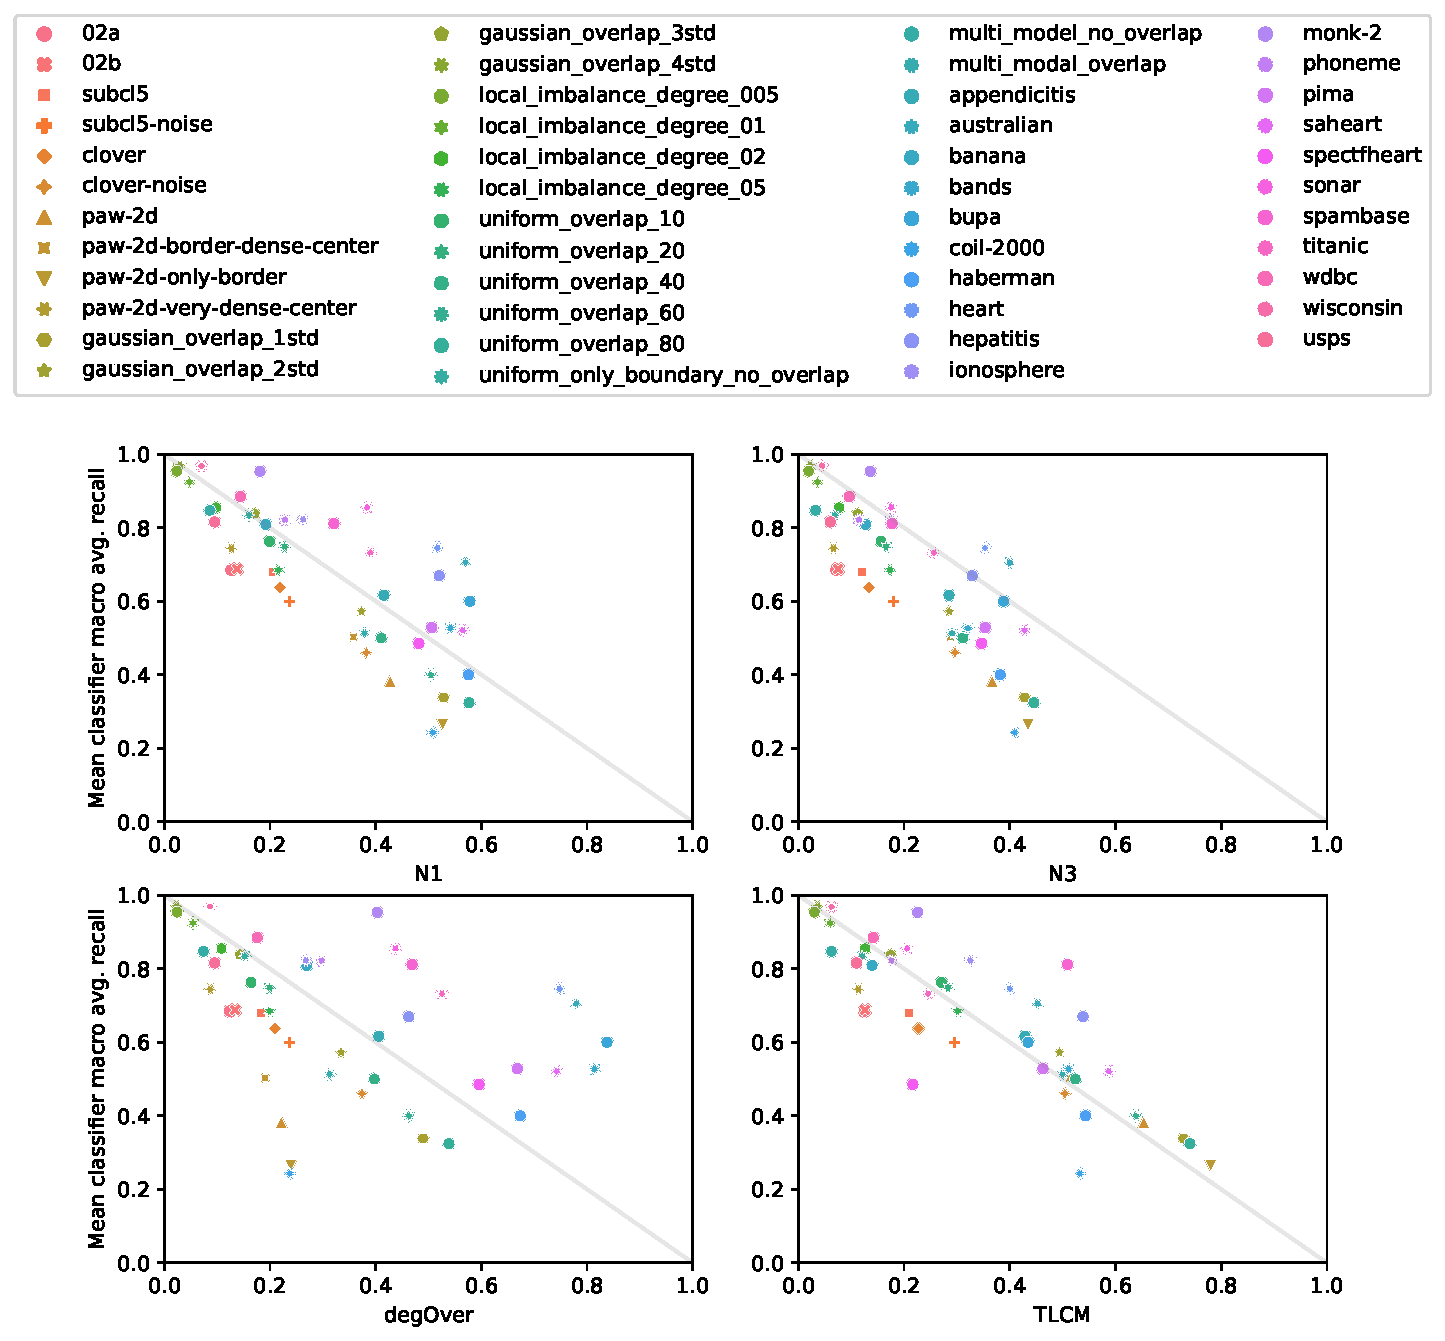
\includegraphics[width=2\columnwidth]{plots/dataset_plots/siam_plot_mac_rec.pdf}
\caption{\label{fig:dataset_plot}The correlation between a mean classifiers performance in terms of macro averaged recall, and the \emph{TLCM} measure.}
\end{figure*}

\begin{table}[]
    \centering
    \begin{tabular}{lrr}
    \toprule
    Measure &  Cor. coef &      p-value \\
    \midrule
         IR &  -0.497220 & 3.772179e-04 \\
         N1 &  -0.773819 & 1.794738e-10 \\
         \emph{N3} &  \emph{-0.844482} & \emph{8.708496e-14} \\
      degIR &  -0.421630 & 3.160467e-03 \\
    degOver &  -0.374425 & 9.517588e-03 \\
       \textbf{TLCM} &  \textbf{-0.852228} & \textbf{3.005538e-14} \\
    \bottomrule
    \end{tabular}
    \caption{\label{tab:mac_rec}Pearson correlation analysis for correlation between macro averaged recall and the complexity measure}
\end{table}

\begin{table}[]
    \centering
    \begin{tabular}{lrr}
    \toprule
    Measure &  Cor. coef &      p-value \\
    \midrule
         IR &  -0.279258 & 5.730783e-02 \\
        \emph{N1} &  \emph{-0.829817} & \emph{5.618854e-13} \\
        \textbf{N3} &  \textbf{-0.850518} & \textbf{3.820528e-14} \\
        degIR &  -0.126509 & 3.967933e-01 \\
        degOver &  -0.552228 & 5.715403e-05 \\
        TLCM &  -0.812841 & 3.945542e-12 \\
    \bottomrule
    \end{tabular}
    \caption{\label{tab:gmean}Pearson correlation analysis for correlation between gmean score and the complexity measure}
\end{table}

\begin{table}[]
    \centering
    \begin{tabular}{lrr}
    \toprule
    Measure &  Cor. coef &      p-value \\
    \midrule
        IR &  -0.469837 & 8.621288e-04 \\
        N1 &  -0.748928 & 1.410436e-09 \\
        \textbf{N3} &  \textbf{-0.781128} & \textbf{9.319564e-11} \\
        degIR &  -0.373966 & 9.612870e-03 \\
        degOver &  -0.384524 & 7.615881e-03 \\
       \emph{TLCM} &  \textit{-0.779805} & \textit{1.051292e-10} \\
    \bottomrule
    \end{tabular}
    \caption{\label{tab:precision}Pearson correlation analysis for correlation between precision and the complexity measure}
\end{table}
In Table \ref{tab:mac_rec},\ref{tab:gmean} and \ref{tab:precision} we have computed the Pearson correlation coefficient between the mean classifiers performance and the Imbalance ratio (IR), the N1 and N3 measure, degIR, degOver and finally the proposed TLCM measure. The corresponding p-value is also presented. Pearson's correlation coefficient measures the linear correlation between the two sets of data, and is normalized to be between -1 and 1. In the Tables we observe negative values approaching -1 which means that there is a linear correlation with a negative sign. In this case, this is the desired behaviour as we want to see a a degradation in classifier performance, as the complexity measure increases. Notice however, that a value of -1 does not mean that the relationship is one to one, i.e. a fall in classifier performance does not yield the same increase in complexity measure. The p-value expresses the probability, that we would have achieved this correlation coefficient if there was no linear correlation, and hence a lower value is better. The row with the best correlation coefficient is highlighted in \textbf{bold} and the second best is \emph{emphasized}. As stated in the Section~\ref{sec:introduction} the de facto standard complexity measure for imbalanced datasets is IR. As shown in the introduction, a visual inspection of the imbalance ratios linear correlation with the mean classifiers' performance Figure~\ref{fig:ir_dataset_plot} is not very clear. This is confirmed for all three quality measures in the correlation tables. In terms of macro averaged recall \ref{tab:mac_rec}, the TLCM measure performs best, with N1 as a close follow up. In terms of gmean scores N3 performs best, N1 second best and TLCM is the third best performer. In terms of precision N3 is number one TLCM number two and N1 is the number three. \JG{Could be interesting to add the statistics on the distance to the cm=1-qm line we are compared to the others} \JG{We also need to show, that we are the most interpretable for all the other measures. Could be done by distance from the cm=1-qm}. Between these three measures the linear correlations are extremely close if we compare to the distances to the other measures in the lineup. The value they return is however not so similar which we can see in Figure~\ref{fig:dataset_plot}.

\section{Discussion}
\label{sec:discussion}
Because of the general linear relation between the performance measures typically used to evaluate class imbalanced problems and the TLCM measure, it would be interesting to determine, what causes the few datasets that are far out of this tendency, to exert such behavior. Given the robustness and performance of these complexity measures a new study should be done, to evaluate whether papers on methods handling the imbalance problem are actually evaluated on complex imbalance problems. A visualization to these imbalance problem handling techniques, could be to show where on the complexity plot a dataset is with respect to a certain benchmark classifier, and then show where it is after the imbalance handling technique has been applied. 

\section{Conclusion}
\label{sec:conclusion}
Since the TLCM measure is the first proposed complexity measure which has a clear linear relationship with respect to mean classifier performance of the form $TLCM=1-(QM)$ where the quality measure can be both macro averaged recall and gmean score it fits well as a substitute to the imbalance ratio, because a score is as easy to interpret, yet holds much more information. 

\section{Contributions}
\begin{itemize}
    \item \textbf{We have made faster n1 and n3 implementations that works in the standard scikit-learn workflow style in Python. That also does not use the Gower distance, like the ImbCol measures.}
    \item \textbf{New TLCM measure}
    \item \textbf{We add a collection of datasets, and add the local imbalance datasets to the collection, so future researchers can think more about new problems than recreating old problems}
\end{itemize}

\newpage
\bibliographystyle{siam}
\bibliography{bib}
\end{document}
